\documentclass[a4paper,12pt]{article}
\usepackage[a4paper,margin=1in]{geometry}
\usepackage[font=small,labelfont=bf]{caption}
\usepackage{amsmath}
\usepackage{amssymb}
\usepackage{bigstrut}
\usepackage{blkarray}
\usepackage{bookmark}
\usepackage{booktabs}
\usepackage{dutchcal}
\usepackage{fancyhdr}
\usepackage{framed}
\usepackage{geometry}  
\usepackage{graphicx}
\usepackage{hyperref}
\usepackage{lastpage}
\usepackage{microtype}
\usepackage{multicol}
\usepackage{multirow}
\usepackage{natbib}
\usepackage{pdfpages}
\usepackage{pifont}
\usepackage{ragged2e}
\usepackage{subcaption}
\usepackage{tabto}
\usepackage{tabularx}
\usepackage{wrapfig}
\usepackage{xcolor}
\usepackage{float}
\usepackage{listings}
\newcommand{\xmark}{\color{red}\ding{53}}%
\newcommand{\cmark}{\color{green}\ding{51}}%
\newcolumntype{Y}{>{\RaggedRight\arraybackslash}X} 
\usepackage{adjustbox}
\setlength{\parindent}{0pt}
\pagestyle{fancy}
\fancyfoot{}
\lhead{\textbf{M. L. Mathiesen} \\
 \textbf{J. Lauritsen}}
\fancyfoot[c]{Page \thepage\ of \pageref{LastPage}}
\newcommand{\red}[1]{\textcolor{red}{\textbf{#1}}}

% \usemintedstyle{xcode}
% \setminted[python]{numbersep = 10pt, bgcolor = lightgrey, breaklines, autogobble, fontsize=\footnotesize, baselinestretch=1.2}


\definecolor{sbase03}{HTML}{002B36}
\definecolor{sbase02}{HTML}{073642}
\definecolor{sbase01}{HTML}{586E75}
\definecolor{sbase00}{HTML}{657B83}
\definecolor{sbase0}{HTML}{839496}
\definecolor{sbase1}{HTML}{93A1A1}
\definecolor{sbase2}{HTML}{EEE8D5}
\definecolor{sbase3}{HTML}{FDF6E3}
\definecolor{syellow}{HTML}{B58900}
\definecolor{sorange}{HTML}{CB4B16}
\definecolor{sred}{HTML}{DC322F}
\definecolor{smagenta}{HTML}{D33682}
\definecolor{sviolet}{HTML}{6C71C4}
\definecolor{sblue}{HTML}{268BD2}
\definecolor{scyan}{HTML}{2AA198}
\definecolor{sgreen}{HTML}{859900}

\usepackage{FiraMono}
\lstdefinestyle{solarized-light}{
  frame=lines,
  xleftmargin=0pt,
  belowcaptionskip=1\baselineskip,
  breaklines=true,
  showstringspaces=false,
  tabsize=1,
  columns=fixed,
  mathescape=true,
  extendedchars=true,
  backgroundcolor=\color{sbase3},
  keywordstyle=\color{scyan},
  stringstyle=\color{sviolet},
  numberstyle=\color{sviolet},
  identifierstyle=\color{sbase03},
  commentstyle=\color{sgreen},
  basicstyle=\color{black}\ttfamily\lst@ifdisplaystyle\footnotesize\fi,
}

% \textbf{\cprotect{\verb|a|}}

\lstnewenvironment{python}
{\lstset{language=Python,style=solarized-light}}
{}

\begin{document}
	\begin{titlepage} % Suppresses displaying the page number on the title page and the subsequent page counts as page 1
		\newcommand{\HRule}{\rule{\linewidth}{0.5mm}} % Defines a new command for horizontal lines, change thickness here
		
		\center % centre everything on the page
		
		%------------------------------------------------
		%	Headings
		%------------------------------------------------
		
		\textsc{\LARGE University of Southern Denmark}\\[0.5cm] % Main heading such as the name of your university/college
		
		\textsc{\Large Dept. of Mathematics \& Computer Science
         }\\[0.5cm] % Minor heading such as course title
		
		%------------------------------------------------
		%	Title
		%------------------------------------------------
		
		\HRule\\[0.2cm]
		
		{\huge\bfseries ISA \\ [0.4cm] Blood donor appointment scheduling
		}\\[0.4cm] % Title of your document
		
		\HRule\\[2 cm]
		
		%------------------------------------------------
		%	Author(s)
		%------------------------------------------------
		
	
		\begin{flushleft}
			\large
			\textit{Authors}\\
			Mikkel Liljegren Mathiesen\\
			\textit{08-10-93}, Mathematics–economics, 9th semester\\
			\ \\
			Johannes Lauritsen\\
			\textit{12-05-95}, Mathematics–economics, 9th semester
			 % Your name
		\end{flushleft}
		
		\begin{flushleft}
			\large
			\textit{Supervisors}\\
			Associate Professor Jacopo Mauro\\
			Postdoc Saverio Giallorenzo
			

			 % Your name
		\end{flushleft}

		% If you don't want a supervisor, uncomment the two lines below and comment the code above
		
		
		%------------------------------------------------
		%	Date
		%------------------------------------------------
		
		\vfill\vfill\vfill % Position the date 3/4 down the remaining page
		
		{\large\today} % Date, change the \today to a set date if you want to be precise
		
		%------------------------------------------------
		%	Logo
		%------------------------------------------------
		
		\vfill\vfill

		%----------------------------------------------------------------------------------------
		
		\vfill % Push the date up 1/4 of the remaining page
		
	\end{titlepage}
	\pagebreak

\thispagestyle{empty}
\newpage
\tableofcontents
\newpage
\setcounter{page}{1}

\textbf{TODO}

\begin{itemize}
    \item \ding{51} Fix background descriptions
    \item \ding{53} Fix research questions
    \item \ding{53} Make SLR more systematic!! (read article?)
    \item \ding{53} Individual contribution
    \item \ding{53} Argue why we didn't use optimization methods
    \item \ding{53} Results (How to present results? What to conclude?)
    \begin{itemize}
        \item \ding{53} Validate simulator (impossible)
        \item \ding{53} Visualize chair occupancy
        \item \ding{53} Visualize staff working
        \item \ding{53} Waiting times data
        \item \ding{53} Inter-arrival time analysis
        \item \ding{53} Discussion of possible improvements
    \end{itemize}
    \item \ding{51} Rewrite Goal
    \item \ding{51} How many nurses?
    \item \ding{51} How many receptions?
\end{itemize}

\newpage

\section{Introduction}

Voluntary blood and plasma donation is an essential part of the healthcare system in Denmark. The blood and plasma are vital in surgery, production of medicine, and many others. But since it is entirely voluntary for the donors, a large percentile does not show up ($\approx 30\%$ for Næstved sygehus, which is the place we consider in this article). The majority of the donors book a time slot online, when a time slot is booked, a bed is blocked in that time slot and cannot be re-assigned to other donors. So if a donor does not show up for an appointment, the hospital loses a precious opportunity to collect life-saving donations. In this project, we will attempt to create a scheduling system that reduces the number of empty donation beds. This is done by implementing an event simulator that simulates what happens in one day in the donation room. The simulator will provide information about each donor: no-show, arrival time, donation time if any errors occur, etc. Then the idea is that our scheduling system will allow overbooking, and the event simulator will provide useful data for when overbooking opportunities arise. In the event simulations, each donor's historical data will be considered, such as no-show rates, donation time, and more.





\subsection{Goal}

The goal is to create a discrete event simulator that is able to simulate a day at the hospital. It should take as input the donors' arrival times and be able to output timestamps for each event in the process (the events in the process can be seen in Figure \ref{flow}).



\subsection{Research questions}

\begin{itemize}
    \item Does this paper use overbooking to accommodate no-shows? If, so does it improve? If not, do they provide a reason for not considering it?
    \item Is this paper talking about donor scheduling? If so, what optimization methods are used?
    \item Does the paper consider donors show up history to predict better whether they will show up in the future?
    \item Does the paper include stochastic methods to describe the real world better?
    \item Does the paper consider walk-in donors? If not, why is that?
\end{itemize}

\section{Background} 

When dealing with scheduling, one way of improving it is by using optimization methods. Some of these methods are described below. In this project, we will, however, focus more on creating an event simulator. After the optimization-section, there will be a brief introduction to discrete event simulation.

\subsection{Optimization}

\subsubsection{Mixed Integer Linear Programming}

The Mixed Integer Linear Programming (MIP) is a handy tool when solving a particular type of problem. The problem type is when the output can only take integer values. For example, when solving a donor scheduling problem, the output can be how many donors we wish to assign to a specific time slot. And since we cannot divide a donor into two, we cannot assign 6.5 donors to a time slot, but instead, 6 or 7 donors would be feasible.

% . Instead, we introduce integer decision variables, possibly alongside real-valued decision variables. Formally, a Mixed Integer Linear Program (MILP) can be defined as follows:
% $$
% \begin{aligned} 
%     \text { maximize } & \quad \mathbf{c}^{T} \mathbf{x} + \mathbf{d}^{T} \mathbf{y} \\
%     \text { subject to } & \quad A \mathbf{x} + B \mathbf{y} \leq \mathbf{b} \\
%     & \quad \mathbf{x} \in \mathbb{R}_{0}^{+} \\
%     & \quad \mathbf{y} \in \mathbb{I}_{0}^{+}
% \end{aligned}
% $$
% where $\mathbf{x}$ is a vector consisting of non-negative continuous variables, $\mathbf{y}$ consist of non-negative integer variables. $A, B$ are $m \times n$ matrix which is given, also $\mathbf{c}, \mathbf{d} \in \mathbb{R}^n$ and $\mathbf{b} \in \mathbb{R}^m$ are given vectors and $\mathbf{0}$ is the zero vector with $n$ entries.

\bigbreak
\subsubsection{\textcolor{red}{Local search (WIP)}}

% The Local Search (LS) method is a way to improve an already existing solution by exploring the neighborhood. By, for example, using the "Hill-climbing search", which for a maximizing (minimization) problem keeps going in the direction of largest increase (decrease). When the local optimum is reached, the algorithm terminates and returns the (possibly better) new solution. This method will never worsen the initially given solution to the LS, but sometimes by worsening the solution, one can reach a better solution. An algorithm that allows a worsening solution is "Simulated annealing", which performs random walks in some direction that very well may lead to a worse solution. But with a maximization (minimization) problem, one can escape a "low peak" ("high valley") and possible reach a better optimum than with a non-worsening LS.

\bigbreak
\subsubsection{Markov Chain}

A Markov Chain (MC) is a very useful instrument when there is a stochastic process involved in a model. A stochastic process could be the probability that a donor shows up. Another stochastic process could be the probability that the collection of blood is a success. Drawing a MC looks very similar to Figure \ref{flow} with the connections between the processes and with what probabilities they are connected. When we are able to connect the processes, we are also able to calculate the probability that a donor successfully will make a donation (i.e., shows up for the appointment, does not get rejected at the reception, and does not fail in the collection process).


% \bigbreak
% Given a sequence of random variables $\{X_1,X_2,...,X_n\}$ and $\{I_1,\dots,I_n\}$ states that satisfy the Markov property, which means that the stochastic process is memoryless. So the probability of moving to the next state only depends on the current state and not on the previous states. Then a discrete-time Markov chain must satisfy the following:

% \[ Pr(X_{n} = x \ | \ X_1 = x_1, \dots , X_{n-1} = x_{n-1}) = Pr(X_{n} = x \ | \ X_{n-1} = x_{n-1}) 
% \]
% An initial starting state $I_0$ has to be defined.


\subsection{Discrete-event simulation}
A discrete-event simulator (DES) is a system that handles events with an underlying discrete-time horizon but can simulate real-life processes that are continuous. An event could, for example, be that a scheduled donor shows up or not. Or a donor successfully donates blood or fails to do so. In a DES, the time horizon is discrete and is called "ticks". The set of these ticks can be described like: $T=\{0,1,2,...,n\}$ and can be modeled as any time unit (hours, minutes, seconds, or even milliseconds). Each event takes a certain amount of ticks; for example, if we implement the ticks as minutes, then the event "Reception" takes approximately three ticks. 


%After each event there will be a change to state of the system. 


\section{Literature review}

An extensive literature review has already been done (see \cite{BD32}) of optimization studies in the healthcare system, which reviews all relevant literature in the years 2003-2016. The paper goes thoroughly through each paper reviewed and categorizes the models used. Then they are able to show the method distribution of the used models. In our literature review, we will include articles also from 2016-2019, which hopefully have new insights in the field. But there will be overlaps in some of the articles since some of the mentioned articles in \cite{BD32} are very relevant for our study.

\bigbreak

\subsection{Method}

The main problem is to improve the current schedule. In the world of healthcare, the word \texttt{appointment} is heavily used. Therefore \texttt{appointment scheduling} must a good starting point for the search string. We also need to take no shows into account; otherwise, we may not be able to compute a good schedule. In the end, this gives us the following search string: \texttt{appointment scheduling no show}. One could probably find a better search string. But for our purpose, it should be sufficient.

\bigbreak

We only have access to the University of Southern Denmark's library of articles. Hence we will only search inside this database (this database includes more than 600 different databases).

\bigbreak

Using our search string, we obtain 51,800 results. This can be reduced significantly by introducing a range for the publishing date. We have chosen to look at publications from the last six years (16/09/2013 - 16/09/2019). This reduced the number of results to 16,233. Using only English publications only reduces the number of results to 16,194. But if we also choose specific disciplines (see figure \ref{search-criteria}), we end up with 2,375 publications.

\bigbreak

\begin{figure}[H]
    \begin{framed}
        \makebox[3.7cm][l]{\textbf{Search string:}} \texttt{appointment scheduling no show} \\
        \makebox[3.7cm][l]{\textbf{Publication date:}} 16/09/2013 - 16/09/2019 (6 years) \\
        \makebox[3.7cm][l]{\textbf{Language:}} English \\
        \makebox[3.7cm][l]{\textbf{Discipline:}} engineering, business, education, applied sciences, computer \\ \makebox[3.7cm][l]{} science, international relations, mathematics, social sciences, \\ \makebox[3.7cm][l]{} statistics, political science, economics
    \end{framed}
    \caption{Search criteria}
    \label{search-criteria}
\end{figure}

\bigbreak

Using our search criteria, we obtain 2,375 results. This is still too many results for us to consider. Therefore we decided to sort the results by \textbf{relevance} and then only look at the first 50 results. We only chose articles with a fitting title, for instance, "Literature review on multi-appointment scheduling problems in hospitals" is excluded due to the term "multi-appointment" as our problem is to make a single appointment for each patient, not a sequence of appointments for each patient.
\bigbreak

The \textbf{relevance} (see \cite{relevance}) is Summons ranking system.  It takes a query (search string) into its algorithm that sorts using Dynamic Rank (depending on the query) and Static Rank (independent on the query). There are many factors under each of these rankings. Some of the most important factors of Dynamic Rank are that it assigns larger weights to an article if the query is included in the title, subtitle, etc. and if it is an exact match, it is even more significant. If a query word is rare, then it is assigned a more substantial weight than a common word. If a query occurs more times in an article, it gets a more significant weight. Some of the essential factors in Static Rank is: Academic content is weighted higher than more common content. Recent articles are weighted higher than old. High citations counts are weighted higher than low counts.

\bigbreak

% At this point, we are left with 42 articles. To reduce this number, we need to read each abstract and exclude the article that does not seem relevant. This left us with 17 articles that are most likely useful to some extent (the exclusion reasoning can be found in Figure \ref{bad}). To further reduce this number, we start reading each article. And when it is clear that the article is either a good or a bad fit, we will sort it as such. After this process, we are left with two fitting articles and 15 unfitting articles (the exclusion reasoning can be found in Figure \ref{semi-good}).

At this point, we are left with 42 articles. To reduce this number, we will introduce seven inclusion criteria, which we will then use to check each article whether they fulfill each of the inclusion criteria.


\subsection{Inclusion criteria}
When reading the articles, we use the following seven inclusion criteria:
\begin{align*}
    a &: \text{Multi-Server} \\
b &: \text{Individual service time} \\
c &: \text{Stochastic service time} \\
d &: \text{Individual no-show probability} \\
e &: \text{Involves simulation} \\
f &: \text{Stochastic arrival time} \\
g &: \text{Focus on no-show} 
\end{align*}

\bigbreak
If an article fulfills at least 5 of 7 criteria, then we will thoroughly read the article and hopefully be able to answer one or more of our research questions.
\begin{figure}[H]
    \centering
    \begin{table}[H]
    \begin{tabularx}{\textwidth}{| @{} c | c | c | c | c | c | c | c | c |}
    \cline{1-8}
    & \multicolumn{7}{c|}{\textbf{Inclusion criteria}}\\
    \cline{1-8}
    \textbf{Publication} & a & b & c & d & e & f & g\\ 
    \cline{1-8}
    \cite{BD29}        & &  &  &  &  &  &\\        \cline{1-8}
    
    \cite{BD25}        &  &  &  &  &  &  & \\       \cline{1-8}
    \cite{BD38}     & \xmark & \cmark & \cmark  & \xmark  & \cmark  & \cmark  & \xmark \\     \cline{1-8}
    \cite{BD06}        & \xmark & \cmark  & \xmark  & \xmark & \cmark & \xmark  & \cmark  \\        \cline{1-8}
    \cite{BD40}        & \xmark  & \cmark  &  \xmark  & \xmark  & \xmark  & \xmark & \cmark \\        \cline{1-8}
    \cite{BD15}     & \xmark & \xmark & \xmark  & \xmark  & \xmark  & \xmark  & \xmark  \\        \cline{1-8}
    \cite{BD31}     &  \xmark & \xmark & \xmark  & \xmark  & \xmark & \xmark &  \cmark \\        \cline{1-8}
    \cite{BD14}        & \xmark & \cmark & \xmark  &  \cmark & \cmark & \xmark  & \cmark  \\        \cline{1-8}
    \cite{BD41}        &  \xmark & \cmark & \cmark  &  \xmark & \cmark & \cmark &  \cmark \\        \cline{1-8}
    \cite{BD09}        & \xmark & \cmark  & \cmark  & \xmark  & \cmark & \xmark  & \xmark  \\        \cline{1-8}
    \cite{BD18}        & \xmark & \cmark  & \cmark  & \xmark & \xmark  & \xmark & \cmark  \\        \cline{1-8}
    \cite{BD42}       & \xmark & \cmark  & \cmark & \xmark  & \xmark      & \xmark  & \cmark \\        \cline{1-8}
    \cite{BD19}         & \xmark & \xmark  & \xmark  & \cmark & \cmark  & \xmark  & \cmark  \\        \cline{1-8}
    \cite{BD48}         & \cmark & \cmark  &  \cmark & \cmark & \cmark & \xmark  & \cmark  \\        \cline{1-8}
    \cite{BD44}         & \cmark & \cmark & \cmark  &  \xmark & \cmark  & \xmark & \cmark  \\        \cline{1-8}
    \cite{BD05}         & \xmark & \cmark & \cmark  & \cmark  & \cmark  & \cmark  & \cmark  \\        \cline{1-8}
    \cite{BD47}        & \xmark & \cmark & \cmark & \xmark &  \cmark & \xmark & \cmark \\        \cline{1-8}
    \cite{BD32}        & \xmark & \xmark &  \xmark&\xmark  &\xmark  &  \xmark& \xmark  \\        \cline{1-8}
    \cite{BD45}        & \xmark &  &  & \xmark & \cmark & \xmark  & \xmark \\        \cline{1-8}
    \cite{BD36}        &  & \cmark & \cmark  & \xmark & \cmark  &  & \xmark \\        \cline{1-8}
    \cite{BD43}        & \cmark & \cmark  & \cmark & \xmark & \cmark & \xmark & \xmark \\        \cline{1-8}
    \cite{BD20}        & \cmark & \cmark & \cmark & \xmark & \xmark & \cmark & \xmark \\        \cline{1-8}
    \cite{BD04}        &\xmark & \cmark & \cmark & \cmark & \cmark & \cmark & \cmark \\        \cline{1-8}
    \cite{BD08}        & \xmark & \cmark & \cmark & \xmark & \xmark & \cmark & \xmark \\        \cline{1-8}
    \cite{BD13}        &\xmark & \cmark & \cmark & \cmark & \xmark & \xmark & \cmark \\        \cline{1-8}
    \cite{BD30}        & \xmark & \cmark & \cmark & \xmark & \cmark & \cmark &  \cmark\\        \cline{1-8}
    \cite{BD23}        & \xmark & \cmark & \cmark & \xmark &\xmark  & \xmark & \cmark \\        \cline{1-8}
    \cite{BD12}        & \xmark & \xmark & \xmark & \cmark & \xmark & \xmark & \cmark \\        \cline{1-8}
    \cite{BD26}      & \xmark & \cmark & \cmark & \cmark & \xmark & \xmark & \cmark \\        \cline{1-8}
    \cite{BD10}        &\xmark & \xmark & \xmark & \cmark & \xmark & \xmark & \cmark \\        \cline{1-8}
    \cite{BD11}        & \xmark & \cmark & \cmark & \xmark & \xmark & \cmark & \cmark \\        \cline{1-8}
    \cite{BD16}        &\xmark &\cmark &\cmark  & \xmark & \xmark & \xmark & \xmark \\        \cline{1-8}
    \cite{BD17}  & \xmark & \xmark & \xmark & \xmark & \xmark & \xmark & \xmark  \\        \cline{1-8}
    \cite{BD21}        & \xmark & \cmark & \cmark &\xmark  &\cmark   & \xmark &\xmark  \\        \cline{1-8}
    \cite{BD22}     & \cmark & \xmark &  \xmark & \xmark & \cmark & \xmark & \xmark \\        \cline{1-8}
    \cite{BD24}&\xmark &  &  & \xmark &  &  \xmark&  \xmark\\        \cline{1-8}
    \cite{BD28}        & &  &  &  &  &  &  \\        \cline{1-8}
    \cite{BD33}        & &  &  &  &  &  &  \\        \cline{1-8}
    \cite{BD34}& &  &  &  &  &  &  \\        \cline{1-8}
    \end{tabularx}
    \end{table}

    \caption{How many inclusion criteria each article fulfills}
    \label{bad}
\end{figure}

Then we look at articles that fulfill at least five of the inclusion criteria.

\begin{figure}[H]
    \begin{center}
    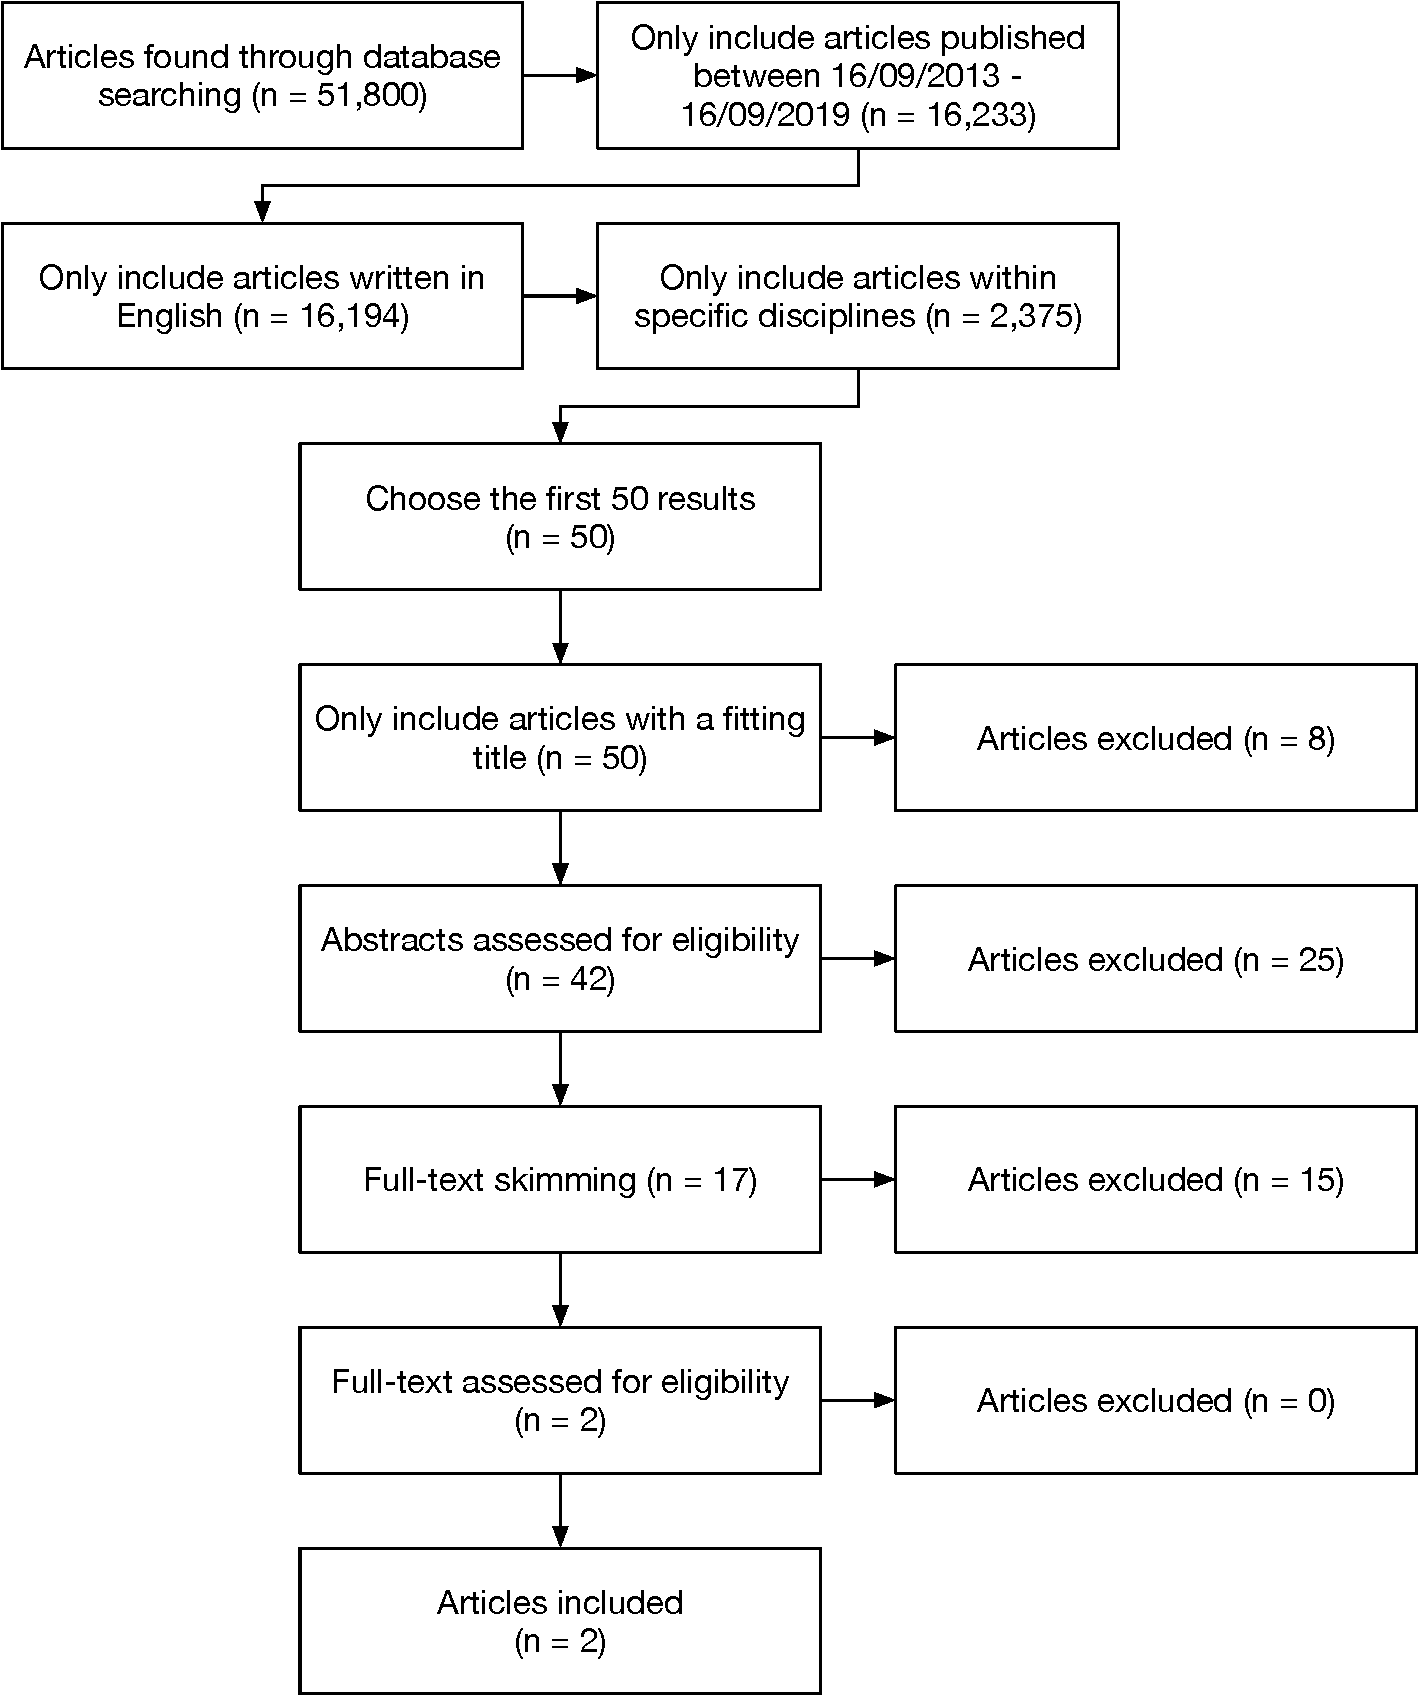
\includegraphics[scale=0.5]{PRISMA.pdf}
    \end{center}
    \caption{PRISMA diagram}
    \label{prisma}
\end{figure}

\subsection{Results}

% \begin{figure}[H]
%     \begin{table}[H]
%     \begin{tabularx}{\textwidth}{@{} c Y @{}}
%     \toprule
%     Publication & Reason \\ \midrule
%     \cite{BD29}        &    They use a Markov decision process that is shown to be weakly coupled. Hence they are able to use the Lagrangian relaxation method. \\
%     \cite{BD25}        &    Aims to find individual no-show probabilities by looking at no-show history. Probabilities are computed by regression-like modeling and functional approximation, using the sum of exponential functions, to produce probability estimates. \\
%     \bottomrule
%     \end{tabularx}
%     \end{table}
%     \caption{Final selection of articles}
%     \label{good}
% \end{figure}

% \begin{figure}[H]
%     \begin{table}[H]
%     \begin{tabularx}{\textwidth}{@{} c Y @{}}
%     \toprule
%     Publication & Reason \\ \midrule
%     \cite{BD38}        &    Single-server queuing model. It requires that the patients have to visit the same doctor and do not accept walk-ins. \\
%     \cite{BD06}        &    Single-server queuing model. \\
%     \cite{BD40}        &    Single-server queuing model. \\
%     \cite{BD15}        &    Single-server queuing model. \\
%     \cite{BD31}        &    Single-server queuing model. \\
%     \cite{BD14}        &    Assumes that all donors have identical service time and the same no-show probability. \\
%     \cite{BD41}        &    Assumes fixed consultation length. This is too restrictive for our problem. \\
%     \cite{BD09}        &    Single-server queuing model. \\
%     \cite{BD18}        &    Takes an analytical approach instead of using simulation techniques (which is what we want) \\
%     \cite{BD42}        &    It is assumed that the service time for each donor is the same, and walk-in donors are not considered. \\
%     \cite{BD19}        &    Giving same-day appointments to likely shows and future-day appointments to likely no-shows. Not useful for our case as we cannot expect donors to accept rescheduling. \\
%     \cite{BD48}        &    Only one no-show probability, which is too restrictive. \\
%     \cite{BD44}        &    Uses health information that we are not provided. \\
%     \cite{BD05}        &    Single-server queuing model. \\
%     \cite{BD47}        &    Considers only one no-show probability, which is too restrictive. \\
%     \bottomrule
%     \end{tabularx}
%     \end{table}
%     \caption{Articles first chosen based on abstract, but then excluded after skimming}
%     \label{semi-good}
% \end{figure}

% \begin{figure}[H]
%     \centering
    
%     \begin{table}[H]
%     \begin{tabularx}{\textwidth}{@{} c Y @{}}
%     \toprule
%     Publication & Reason \\ \midrule
%     \cite{BD32}        &    This is a literature review in the outpatient appointment system in healthcare of many optimization studies, which gives a great overview of the literature but does not help in directly solving our problem.  \\
%     \cite{BD45}        &    Account for patient choices in order to improve patient satisfaction. Computes a complete set of appointments that donors can then book from. No-show is not considered. \\
%     \cite{BD36}        &    Single-server queuing model. \\
%     \cite{BD43}        &    Free patient from blind waits. Not relevant for our study as we expect the vast majority of donors to be unwilling to wait. Single-server queuing model. \\
%     \cite{BD20}        &    Allows for urgent patients. Not directly applicable to our study. \\
%     \cite{BD04}        &    Single server queuing model. Customers are assumed to arrive deterministically. \\
%     \cite{BD08}        &    It does not account for no-shows. \\
%     \cite{BD13}        &    Single-server queuing model. \\
%     \cite{BD30}        &    It uses different characteristics of individual patients to estimate examination time, several pieces of information are needed to implement this, many of which we do not have for our problem. \\
%     \cite{BD23}        &    Single-server queuing model. \\
%     \cite{BD12}        &    Assumes a constant service time for each donor. \\
%     \cite{BD26}        &    Choose how early a patient can make a booking. Interesting as there is likely correspondence between no-shows and how soon a booking was made. Uses a single server queuing model. \\
%     \cite{BD10}        &    The article only investigates the problem of donor cancellations and no-shows but does not solve the problem with scheduling. \\ 
%     \cite{BD11}        &    A single-server queuing model. \\
%     \cite{BD16}        &    The article does not consider no-shows and only looks at a single day,  but many donors prefer different days in the week, which we would like to include in our model.  \\
%     \cite{BD17}        &    The article does not consider no-shows and walk-in donors, which we would like to include in our model.  \\
%     \cite{BD21}        &    The article does not consider no-shows and walk-in donors, which we would like to include in our model.\\
%     \cite{BD22}        &    The article considers patient preferences to different physicians, which does not fit our approach. \\
%     \cite{BD24}        &    The article considers the same no-show probability for all donors. \\
%     \cite{BD28}        &    The article does not consider donors to "drop-in" without an appointment, which we have to consider. \\
    
%     \cite{BD33}        &    The article does not solve the BD scheduling problem but instead discuss some of the literature and unaddressed problems in the field. \\ 
%     \cite{BD34}        &    The article limits the number of days a donor can book an appointment time in advance, which we are not interested in. \\
%     \bottomrule
%     \end{tabularx}
%     \end{table}

%     \caption{Omitted articles based on abstract}
%     \label{bad}
% \end{figure}

% \begin{figure}[H]
% \ContinuedFloat
%     \centering

%     \begin{table}[H]
%     \begin{tabularx}{\textwidth}{@{} c Y @{}}
%     \toprule
%     Publication & Reason \\ \midrule
%     \cite{BD35}        &    The article considers a single server problem and assume a constant service time for all donors. No-shows are also neglected. \\
%     \cite{BD37}        &    The article sets the no-show rate to a fixed constant for all donors; in our model, we would like to be able to distinguish between each donor. \\
%     \cite{BD46}        &    The article has its focus on donors' unpunctuality; our focus is more on donors being no-shows.  \\
%     \bottomrule
%     \end{tabularx}
%     \end{table}

%     \caption{Omitted articles based on abstract}
%     \label{bad}
% \end{figure}

\subsection{Discussion}

% \textcolor{red}{\textbf{Summarise and discuss the findings and conclusions of the review in a balanced and impartial way, in the context of previous theory, evidence and practice}}

Most articles consider the single-server queueing model. This is not what we want, as we have more than one chair in the clinic. In fact, there are up to 11 chairs available (7 for plasma and 4 for blood). Some articles consider a fixed no-show rate; this is not what we want since we have data on each donor and would like to have different no-show rates for each donor. Some articles have constant service time for each donor; this is not what we want - instead, we want a stochastic service time since this is more realistic. Some articles do not consider walk-ins, but we would like to take into account a stochastic amount of walk-ins since this is more realistic.

%\textcolor{red}{\textbf{Explicitly and intuitively link your conclusions to the evidence reviewed}}

%\textcolor{red}{\textbf{Discuss the strengths and limitations of the literature and, by implication, the review, including considering the scientific quality of included studies and methodological problems in the literature (e.g., methodological rigor or lack thereof, the amount of evidence, its consistency, and its methodological diversity). Conclusions should be tempered by the flaws and weaknesses in the evidence. Perhaps propose a new conceptualisation or theory which accounts for inconsistencies. (Baumeister & Leary, 1997)}}

%\textcolor{red}{\textbf{Establish to what extent existing research has progressed towards clarifying a particular problem/formulate general statements or an overarching conceptualization. Quantitative or qualitative reviews may conclude that the available evidence suggests one of four possibilities (see Baumeister & Leary, 1997, for a detailed discussion of these)}}

%\textcolor{red}{\textbf{Comment on, evaluate, extend, or develop theory}}

%\textcolor{red}{\textbf{Draw conclusions and make recommendations for practice}}

%\textcolor{red}{\textbf{Describe directions for future theory, evidence and practice by pointing out remaining unresolved issues}}


\section{EXAMPLE OF PYTHON CODE}

\begin{python}
    # Python program for implementation of MergeSort 
  
# Merges two subarrays of arr[]. 
# First subarray is arr[l..m] 
# Second subarray is arr[m+1..r] 
def merge(arr, l, m, r): 
    n1 = m - l + 1
    n2 = r- m 
  
    # create temp arrays 
    L = [0] * (n1) 
    R = [0] * (n2) 
  
    # Copy data to temp arrays L[] and R[] 
    for i in range(0 , n1): 
        L[i] = arr[l + i] 
  
    for j in range(0 , n2): 
        R[j] = arr[m + 1 + j] 
  
    # Merge the temp arrays back into arr[l..r] 
    i = 0     # Initial index of first subarray 
    j = 0     # Initial index of second subarray 
    k = l     # Initial index of merged subarray 
  
    while i < n1 and j < n2 : 
        if L[i] <= R[j]: 
            arr[k] = L[i] 
            i += 1
        else: 
            arr[k] = R[j] 
            j += 1
        k += 1
  
    # Copy the remaining elements of L[], if there 
    # are any 
    while i < n1: 
        arr[k] = L[i] 
        i += 1
        k += 1
  
    # Copy the remaining elements of R[], if there 
    # are any 
    while j < n2: 
        arr[k] = R[j] 
        j += 1
        k += 1
  
# l is for left index and r is right index of the 
# sub-array of arr to be sorted 
def mergeSort(arr,l,r): 
    if l < r: 
  
        # Same as (l+r)/2, but avoids overflow for 
        # large l and h 
        m = (l+(r-1))/2
  
        # Sort first and second halves 
        mergeSort(arr, l, m) 
        mergeSort(arr, m+1, r) 
        merge(arr, l, m, r) 
  
  
# Driver code to test above 
arr = [12, 11, 13, 5, 6, 7] 
n = len(arr) 
print ("Given array is") 
for i in range(n): 
    print ("%d" %arr[i]), 
  
mergeSort(arr,0,n-1) 
print ("\n\nSorted array is") 
for i in range(n): 
    print ("%d" %arr[i]), 
}
\end{python}

\bigbreak

\section{Process description}

The blood/plasma donation can be seen in Figure \ref{flow}. At the initial stage, the plasma and blood donors are scheduled. At the next stage, the donor either shows up or doesn't with different probabilities depending on the donor type. If a donor is a no-show, they exit the system; the remaining donors continue to the next step. The next step is filling out their health information, which approximately takes 5 minutes. Afterward, they are interviewed by the reception (a nurse), which takes approximately 3 minutes; approximately 1.47\%/0.48\% gets rejected of the blood and plasma donors, respectively. Then the nurse will prepare a chair for the donor, and afterward, the needle insertion takes place (this process takes approximately 2 minutes). Then the collection of blood/plasma takes place, which approximately takes 15/45 minutes, respectively. Different factors might cause the collection process to fail; approximately 5.45\%/2.61\% fails the collection process for blood and plasma donors, respectively. If a donor fails the collections process, then they also get the opportunity to rest. If the collection is successful, then the nurse checks the donor's ID, which takes less than 1 minute. Then the donor can rest and depend on the donation type; it approximately takes 10 and 1 minutes for blood and plasma donation, respectively). When the donor is ready, they exit the system. Then the terminal stage occurs for which the nurse prepares the chair for the next donor, and this takes approximately 1 and 4 minutes for blood and plasma donation, respectively.

\begin{figure}[H]
    \begin{center}
    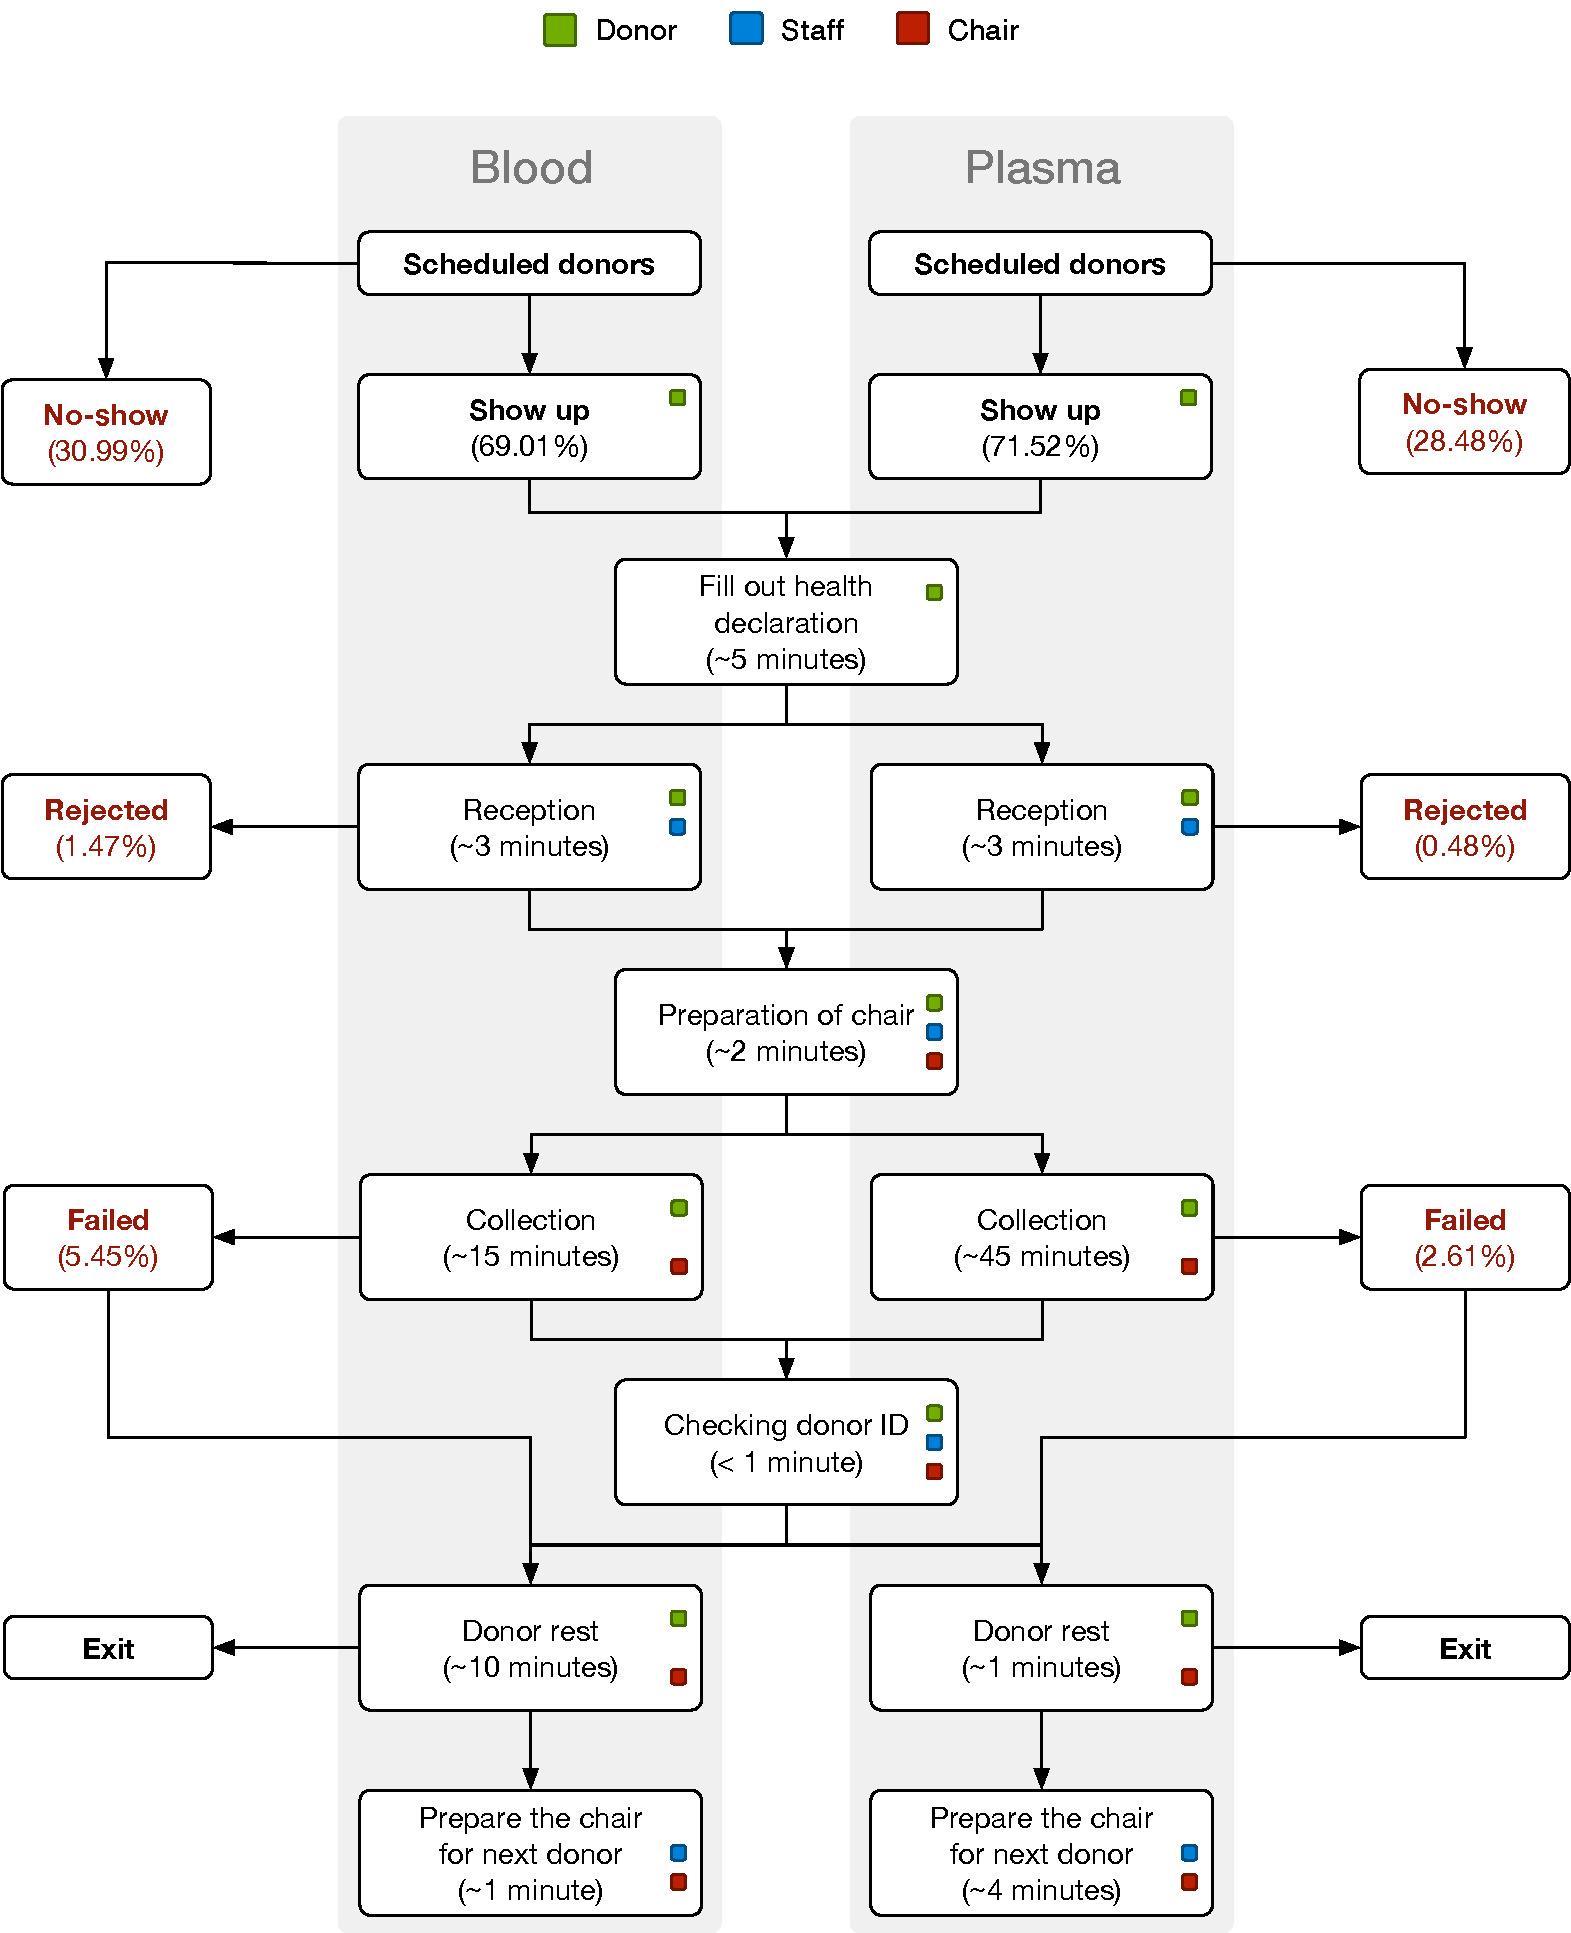
\includegraphics[scale=0.58]{process.pdf}
    \end{center}
    \caption{Process description graph}
    \label{flow}
\end{figure}

\bigbreak
\section{Data}

We have been provided with different spreadsheets containing data from the daily operation in the donor clinic from 2014-01-02 to 2019-08-19.

\bigbreak

Unfortunately, the hospital does not register timestamps for every step in the donation process. Instead, they only record when the donor gets into the reception and then when the collected blood/plasma is registered in the system (which is not necessarily when the donor leaves the chair).
We have been provided with collection times for a subset of the data (12{,}380 out of 53{,}140 rows). The collection times are registered manually by the staff. Hence we can expect to find errors due to human interaction. Out of the 12{,}380 records, only 595 are from blood donations, where the remaining 11{,}785 are plasma donations.


\section{Simulation model}

Due to the missing timestamps in the provided data, it is impossible to create a precise model, as we have to guess which distributions to apply to each of the steps.

\bigbreak

We were provided with approximate completion times for each of the steps in the process (so these times are not based on the provided datasets, but rather a qualified guess on the actual time spent). For each of the steps, we used a Gaussian distribution with the mean set to the approximate completion time and variance set to $1/4$th of the mean.
We can fit the collections times from the dataset to a Gaussian distribution or using kernel density estimation with a Gaussian kernel to obtain a better representation of the underlying data. We can do the same for the inter-arrival time of the donors (under the assumption that the donors use roughly the same amount of time filling out the health declaration, as the first timestamp we have are after the donor has filled out the health declaration). The fitting is done for blood and plasma separately. We also consider successful and failed donations separately, as failed donations often are terminated much faster than successful ones. Comparisons of the two fitting methods can be seen in figures \ref{firstfit}-\ref{lastfit}. It is easy to see that the kernel density estimator with a Gaussian kernel does a much better job at describing the underlying data, hence it is those distributions we will sample from in the simulator.

\begin{figure}[H]
    \begin{minipage}[t]{0.5\textwidth}
        \centering
        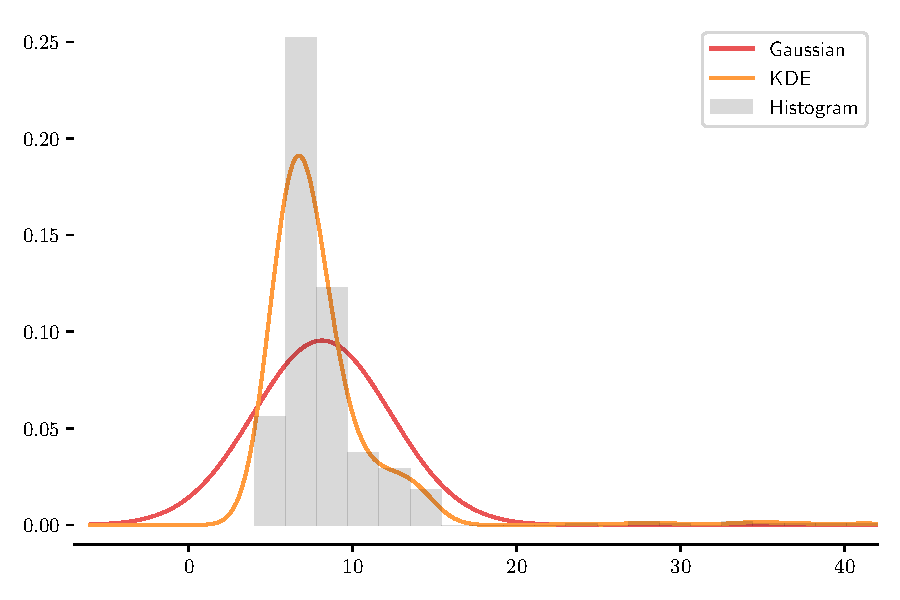
\includegraphics[scale=0.48]{blood_collection_time.pdf}
        \begin{minipage}[t]{0.9\textwidth}
            \centering
            \caption{Fitting distributions to collection time of blood donors that successfully donate}
            \label{firstfit}
        \end{minipage}
    \end{minipage}%
    \begin{minipage}[t]{0.5\textwidth}
        \centering
        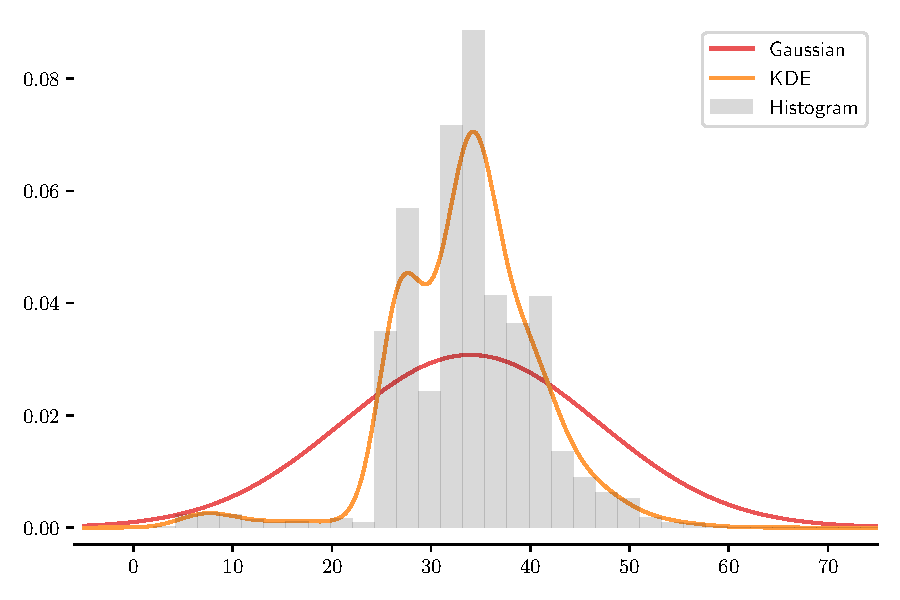
\includegraphics[scale=0.48]{plasma_collection_time.pdf}
        \begin{minipage}[t]{0.9\textwidth}
            \centering
            \caption{Fitting distributions to collection time of plasma donors that successfully donate}
        \end{minipage}
    \end{minipage}
\end{figure}

\begin{figure}[H]
    \begin{minipage}[t]{0.5\textwidth}
        \centering
        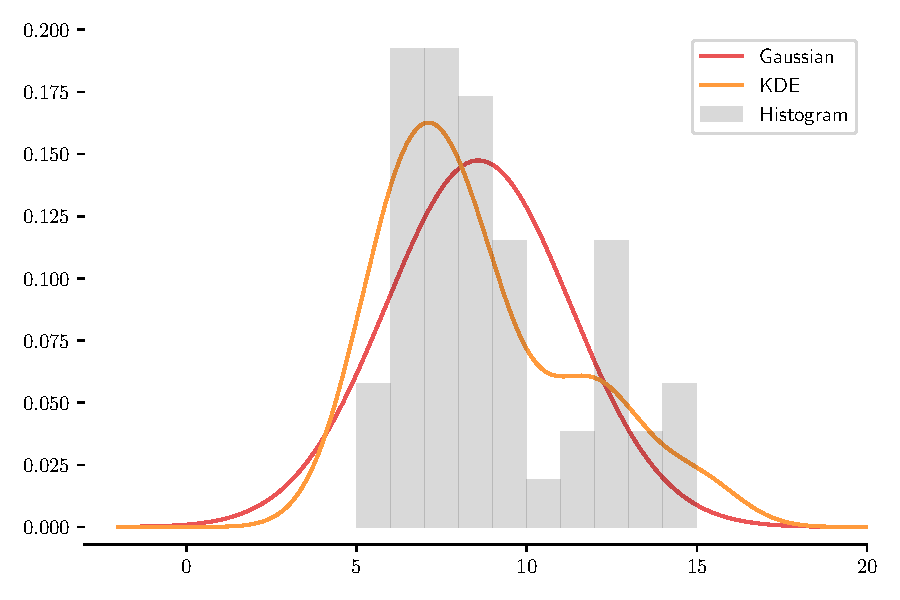
\includegraphics[scale=0.48]{blood_failed_collection_time.pdf}
        \begin{minipage}[t]{0.9\textwidth}
            \centering
            \caption{Fitting distributions to collection time of blood donors that failed}
        \end{minipage}
    \end{minipage}%
    \begin{minipage}[t]{0.5\textwidth}
        \centering
        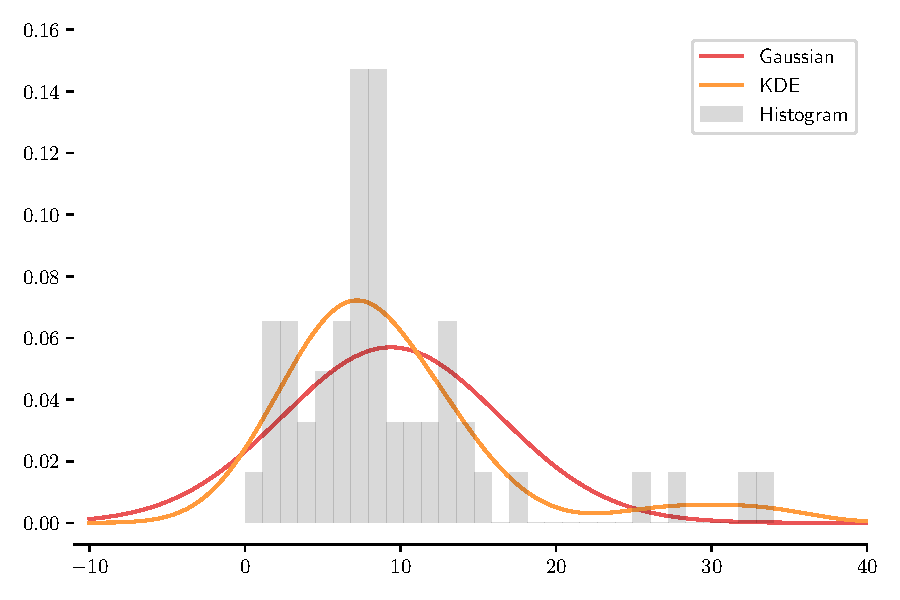
\includegraphics[scale=0.48]{plasma_failed_collection_time.pdf} % kom igang
        \begin{minipage}[t]{0.9\textwidth}
            \centering
            \caption{Fitting distributions to collection time of plasma donors that failed}
        \end{minipage}
    \end{minipage}
\end{figure}

\begin{figure}[H]
    \begin{minipage}[t]{0.5\textwidth}
        \centering
        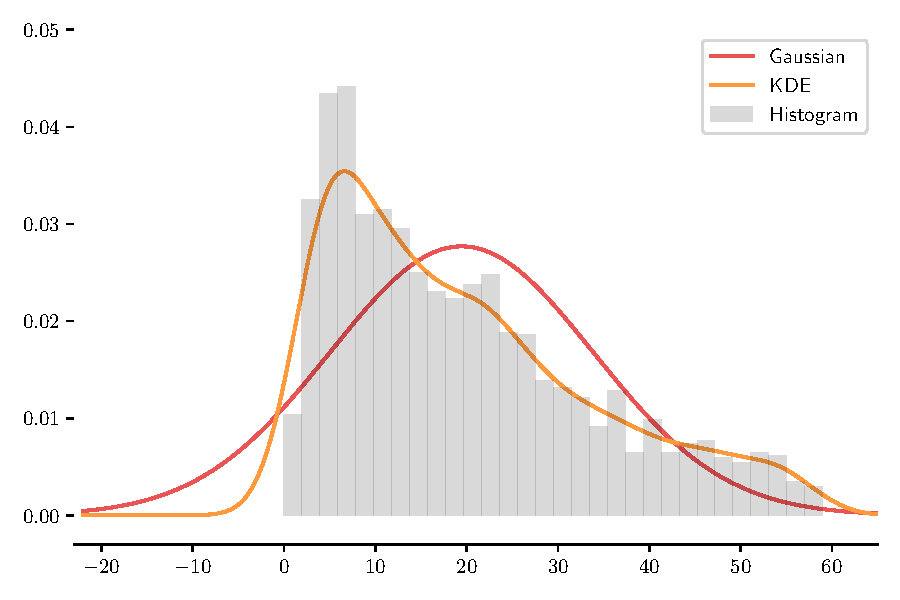
\includegraphics[scale=0.48]{blood_interarrival_time.pdf}
        \begin{minipage}[t]{0.9\textwidth}
            \centering
            \caption{Fitting distributions to inter-arrival times of blood donors}
        \end{minipage}
    \end{minipage}%
    \begin{minipage}[t]{0.5\textwidth}
        \centering
        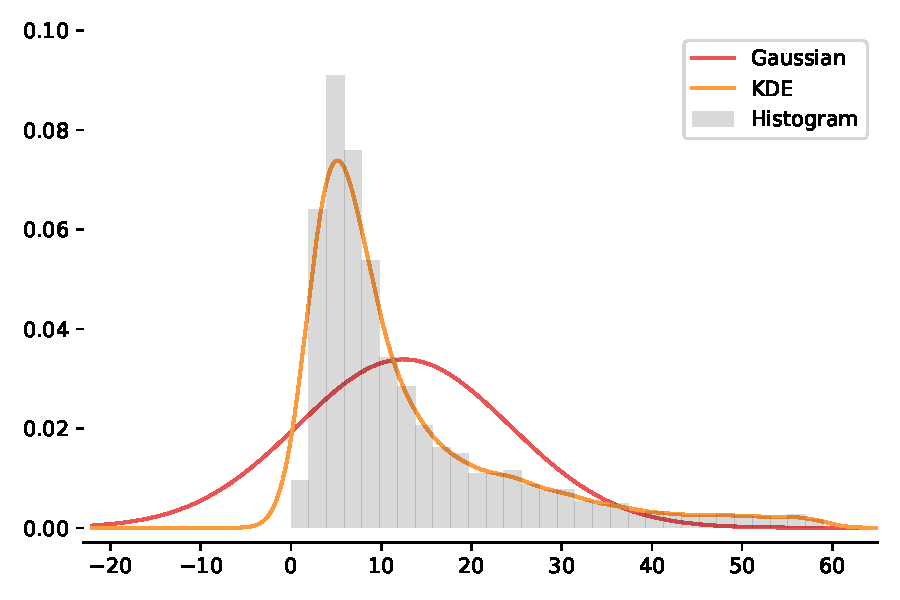
\includegraphics[scale=0.48]{plasma_interarrival_time.pdf}
        \begin{minipage}[t]{0.9\textwidth}
            \centering
            \caption{Fitting distributions to inter-arrival times of plasma donors}
            \label{lastfit}
        \end{minipage}
    \end{minipage}
\end{figure}

\bigbreak

We will use Discrete Event Simulation (DES) to simulate a day in the clinic. To implement the simulator we will use Python and the package \texttt{salabim}.

\bigbreak

In the simulator, blood and plasma donors are spawned in parallel. Donors are spawned according to samples drawn from their respective inter-arrival distribution. After being spawned, the donor will follow the process description graph from the point "Scheduled donors".

\bigbreak

\red{Should we include the code for the simulator here? Or should we show pseudo code?}

\section{Results}

We are not able to compare our model with the data from Næstved.

\begin{figure}[H]
    \begin{center}
    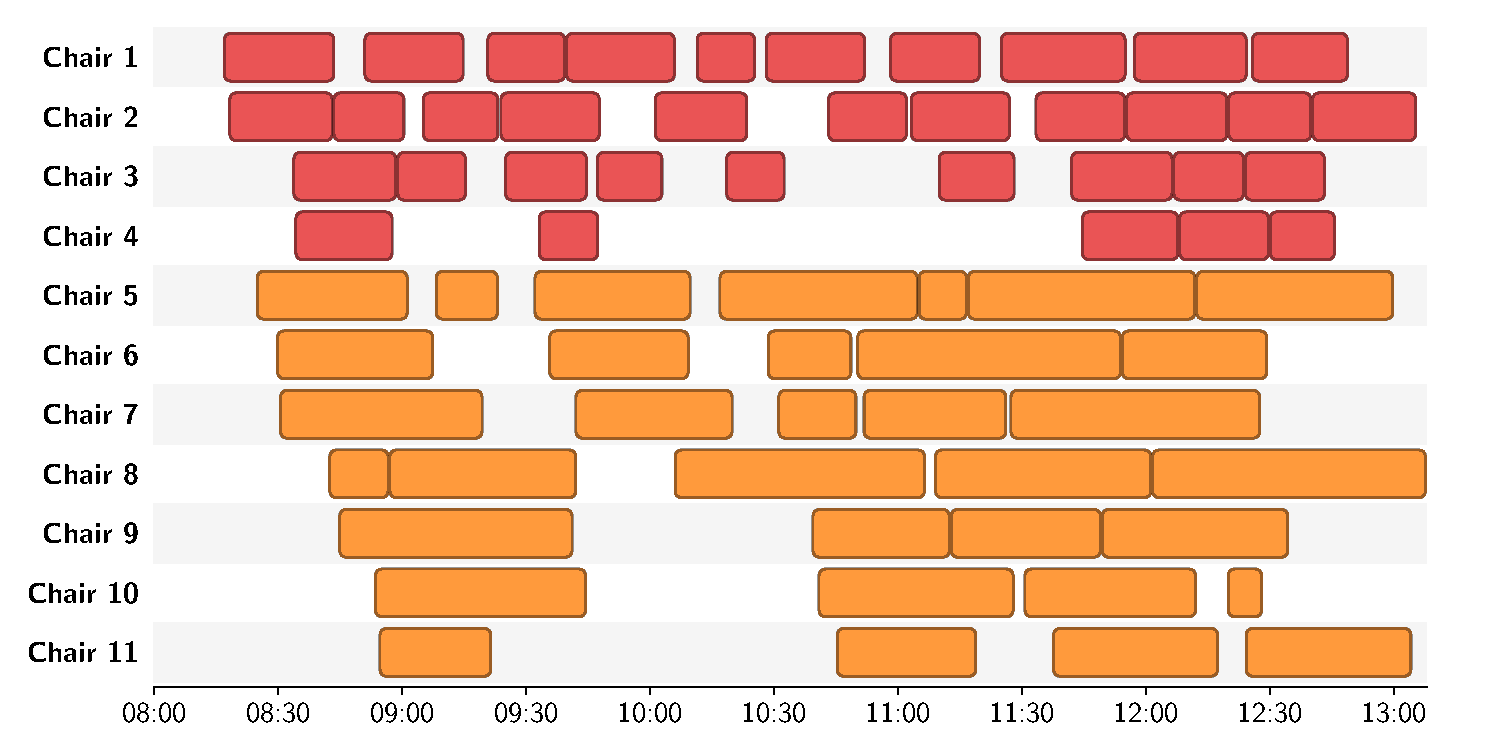
\includegraphics[scale=0.62]{schedule.pdf}
    \end{center}
    \caption{Chair occupancy on a day in the clinic. Red are chairs for blood donation, and orange are chairs for plasma donation.}
    \label{flow}
\end{figure}

\section{Conclusion}

If we were able to obtain timestamps for each of the steps in the donation process, we could implement a much more precise model.

\textbf{Further research:} It should be possible to use some optimization methods after using the event simulator to further improve the scheduling. 
\newpage

\bibliographystyle{unsrt}
\bibliography{bibliography}

\end{document}
